\documentclass[11pt]{article}

% ---------- Packages ----------
\usepackage[a4paper,margin=1in]{geometry}
\usepackage{array}
\usepackage{amsmath}
\usepackage{amssymb}
\usepackage{amsthm}
\usepackage{enumitem}
\usepackage{fancyhdr}
\usepackage{graphicx}
\usepackage{booktabs}
\usepackage{caption}
\usepackage{threeparttable}
\usepackage[hidelinks]{hyperref}

% ---------- Header / Footer ----------
\pagestyle{fancy}
\fancyhf{}
\lhead{\textbf{\course}}
\chead{\textbf{Homework \hwno}}
\rhead{\textbf{\name}}
\cfoot{\thepage}

% ---------- Custom Info ----------
\newcommand{\course}{Time Series Analysis}
\newcommand{\hwno}{2}
\newcommand{\name}{Your Name}
\newcommand{\studentid}{Student ID}
\newcommand{\due}{Due: 2026-03-30}

% ---------- Environments ----------
\newcounter{problem}
\newenvironment{problem}[1][]{
	\refstepcounter{problem}
	\vspace{0.75em}
	\noindent\textbf{Problem \theproblem.} \textit{#1}\par
	\vspace{0.25em}
}{\vspace{0.5em}}

\newenvironment{reference}{
	\noindent\textbf{Reference}\par
}{\vspace{0.75em}}

% ---------- Title Block ----------
\title{\vspace{-1.5em}\textbf{\course} \\ \large Homework \hwno}
\author{\name \quad (\studentid) \\ \due}
\date{}

\begin{document}
	\maketitle
	\vspace{-1em}
	\hrule
	\vspace{1em}
	\begin{problem}
		This problem examines several standard issues in empirical macroeconomics using Chinese macroeconomic data, including the construction of GDP measures, seasonal adjustment, and trend-cycle decomposition. In answering the questions, state your procedures clearly and provide brief economic interpretation where appropriate.
		
		\begin{enumerate}[label=(\alph*)]
			\item Using China’s quarterly GDP data, construct and compare nominal GDP, real GDP, and the corresponding growth measures. In particular, explain the relationship between cumulative series and quarterly flow series, the interpretation of constant-price measures, and the distinction between year-on-year growth rates and cumulative year-on-year growth rates. Based on your results, discuss the different uses of these indicators in macroeconomic analysis.
			
			\item Using China’s real GDP series at 2020 constant prices, carry out seasonal adjustment and use the adjusted series to study short-run fluctuations in economic activity. You may employ the seasonal adjustment methods introduced in class and, where appropriate, compare the resulting adjusted series across alternative procedures. Based on the seasonally adjusted series, compute quarter-on-quarter growth rates or log quarter-on-quarter growth rates, and use both quarter-on-quarter and year-on-year measures to characterize the main phases of China’s macroeconomic fluctuations and major turning points.
			
			\item Using the same real GDP series, apply the Hodrick-Prescott (HP), Baxter-King (BK), and Christiano-Fitzgerald (CF) filters to decompose output into trend and cyclical components. Compare the decomposition results across methods, with particular attention to the estimated trend and cycle. On this basis, construct measures of potential output and the output gap, and compare the output gap with an inflation indicator in order to discuss the possible relationship between real activity and inflationary pressure.
		\end{enumerate}
	\end{problem}
	
	\begin{table}[htbp]
		\small
		\centering
		\caption{Selected Variables From the CEIC Database}
		\label{tab:VariablesCN}
		\begin{threeparttable}
			\renewcommand{\arraystretch}{1}
			\begin{tabular}{cllc}
				\toprule
				ID & Variable 	& Description 										& Frequency \\
				\midrule
				1  & NGDP       & Nominal Gross Domestic Product         		    & Quarterly \\
				2  & NGDPA      & Nominal Gross Domestic Product: AC                & Quarterly \\
				3  & RGDP     	& Real Gross Domestic Product: 2020 Constant Prices & Quarterly \\
				4  & RGDPYoY    & Real Gross Domestic Product Growth: YoY           & Quarterly \\
				5  & RGDPYoYA  	& Real Gross Domestic Product Growth: YoY: AC       & Quarterly \\
				6  & RGDPQoQSA  & Real Gross Domestic Product Growth: QoQ: SA	 	& Quarterly \\
				7  & RIAVYoY   	& Real Industrial Value Added Growth: YoY           & Monthly   \\
				8  & RIAVYoYA  	& Real Industrial Value Added Growth: YoY: AC       & Monthly   \\
				9  & RIAVMoMSA  & Real Industrial Value Added Growth: MoM: SA 		& Monthly   \\
				10 & NRSG      	& Nominal Retail Sale of Consumer Goods             & Monthly   \\
				11 & NRSGYoY    & Nominal Retail Sale of Consumer Goods: YoY        & Monthly   \\
				12 & NRSGYoYA   & Nominal Retail Sale of Consumer Goods: YoY: AC    & Monthly   \\
				13 & NRSGMoMSA  & Nominal Retail Sale of Consumer Goods: MoM: SA 	& Monthly   \\
				14 & CPIYoY    	& Consumer Price Index: YoY 						& Monthly   \\
				15 & CPIMoM    	& Consumer Price Index: MoM  						& Monthly   \\
				\bottomrule
			\end{tabular}
			\begin{tablenotes}[flushleft]
				\footnotesize
				\item \textit{Notes}: YoY, QoQ, and MoM denote year-on-year, quarter-on-quarter, and month-on-month growth rates, respectively. AC indicates accumulated values, while SA indicates seasonally adjusted series.
			\end{tablenotes}
		\end{threeparttable}
	\end{table}


	\begin{problem}
		This problem uses the U.S. FRED-MD database to examine several common steps in applied macroeconomic time-series analysis, including stationarization, outlier treatment, standardization, and the extraction of common movements from a large macroeconomic dataset. Briefly explain the statistical purpose of each procedure and its role in empirical work.
		
		\begin{enumerate}[label=(\alph*)]
			\item Using the FRED-MD dataset, transform the raw series according to the TCODE rules recommended in the original reference. Explain the rationale and statistical meaning of the different transformations, and discuss why stationarization is typically required for subsequent time-series analysis and econometric modeling.
			
			\item After transforming the data, identify and treat extreme observations, and compare the main features of the series before and after outlier adjustment. You may use a robust criterion such as the interquartile range (IQR) rule to detect unusually large observations. Based on the evidence, discuss the periods in which extreme macroeconomic fluctuations are most apparent in the United States, and explain the role of outlier treatment and standardization in multivariate macroeconomic analysis.
			
			\item Building on the preceding data preparation, examine the relationship between U.S. monthly macroeconomic indicators and quarterly GDP fluctuations. You may estimate a dynamic factor model to extract a common factor from the monthly series and compare it with quarterly GDP growth. Based on the results, discuss whether higher-frequency monthly information contains useful signals about broader quarterly economic conditions and whether it may help describe or predict fluctuations in aggregate output (Optional).
		\end{enumerate}
	\end{problem}
	
	\begin{table}[htbp]
		\small
		\centering
		\caption{Selected Variables From the FRED Dataset}
		\label{tab:VariablesUS}
		\begin{threeparttable}
			\renewcommand{\arraystretch}{1}
			\begin{tabular}{cllcc}
				\toprule
				ID & FRED & Description & Frequency & TCODE \\
				\midrule
				1  & GDPC1           & Real Gross Domestic Product                & Quarterly & 5 \\
				2  & RPI             & Real Personal Income                       & Monthly   & 5 \\
				3  & INDPRO          & Industrial Production: Index               & Monthly   & 5 \\
				4  & CUMFNS          & Capacity Utilization: Manufacturing        & Monthly   & 2 \\
				5  & CE16OV          & Civilian Employment                        & Monthly   & 5 \\
				6  & PAYEMS          & All Employees: Total Nonfarm               & Monthly   & 5 \\
				7  & UNRATE          & Civilian Unemployment Rate                 & Monthly   & 2 \\
				8  & DPCERA3M086SBEA & Real Personal Consumption Expenditures     & Monthly   & 5 \\
				9  & RETAILx         & Retail and Food Services Sales             & Monthly   & 5 \\
				10 & UMCSENTx        & Consumer Sentiment Index                   & Monthly   & 2 \\
				11 & S\&P 500        & S\&P's Common Stock Price Index: Composite & Monthly   & 5 \\
				\bottomrule
			\end{tabular}
			\begin{tablenotes}[flushleft]
				\footnotesize
				\item \textit{Notes}: The column \texttt{TCODE} denotes the following data transformation for a series $x$: (1) no transformation; (2) $\Delta x_t$; (3) $\Delta^2 x_t$; (4) $\log(x_t)$; (5) $\Delta \log(x_t)$; (6) $\Delta^2 \log(x_t)$; (7) $\Delta (x_t/x_{t-1} - 1.0)$. The \texttt{FRED} column gives mnemonics in FRED followed by a short description.
			\end{tablenotes}
		\end{threeparttable}
	\end{table}
	
	\newpage
	
	\begin{reference}
		\begin{figure}[htbp]
			\centering
			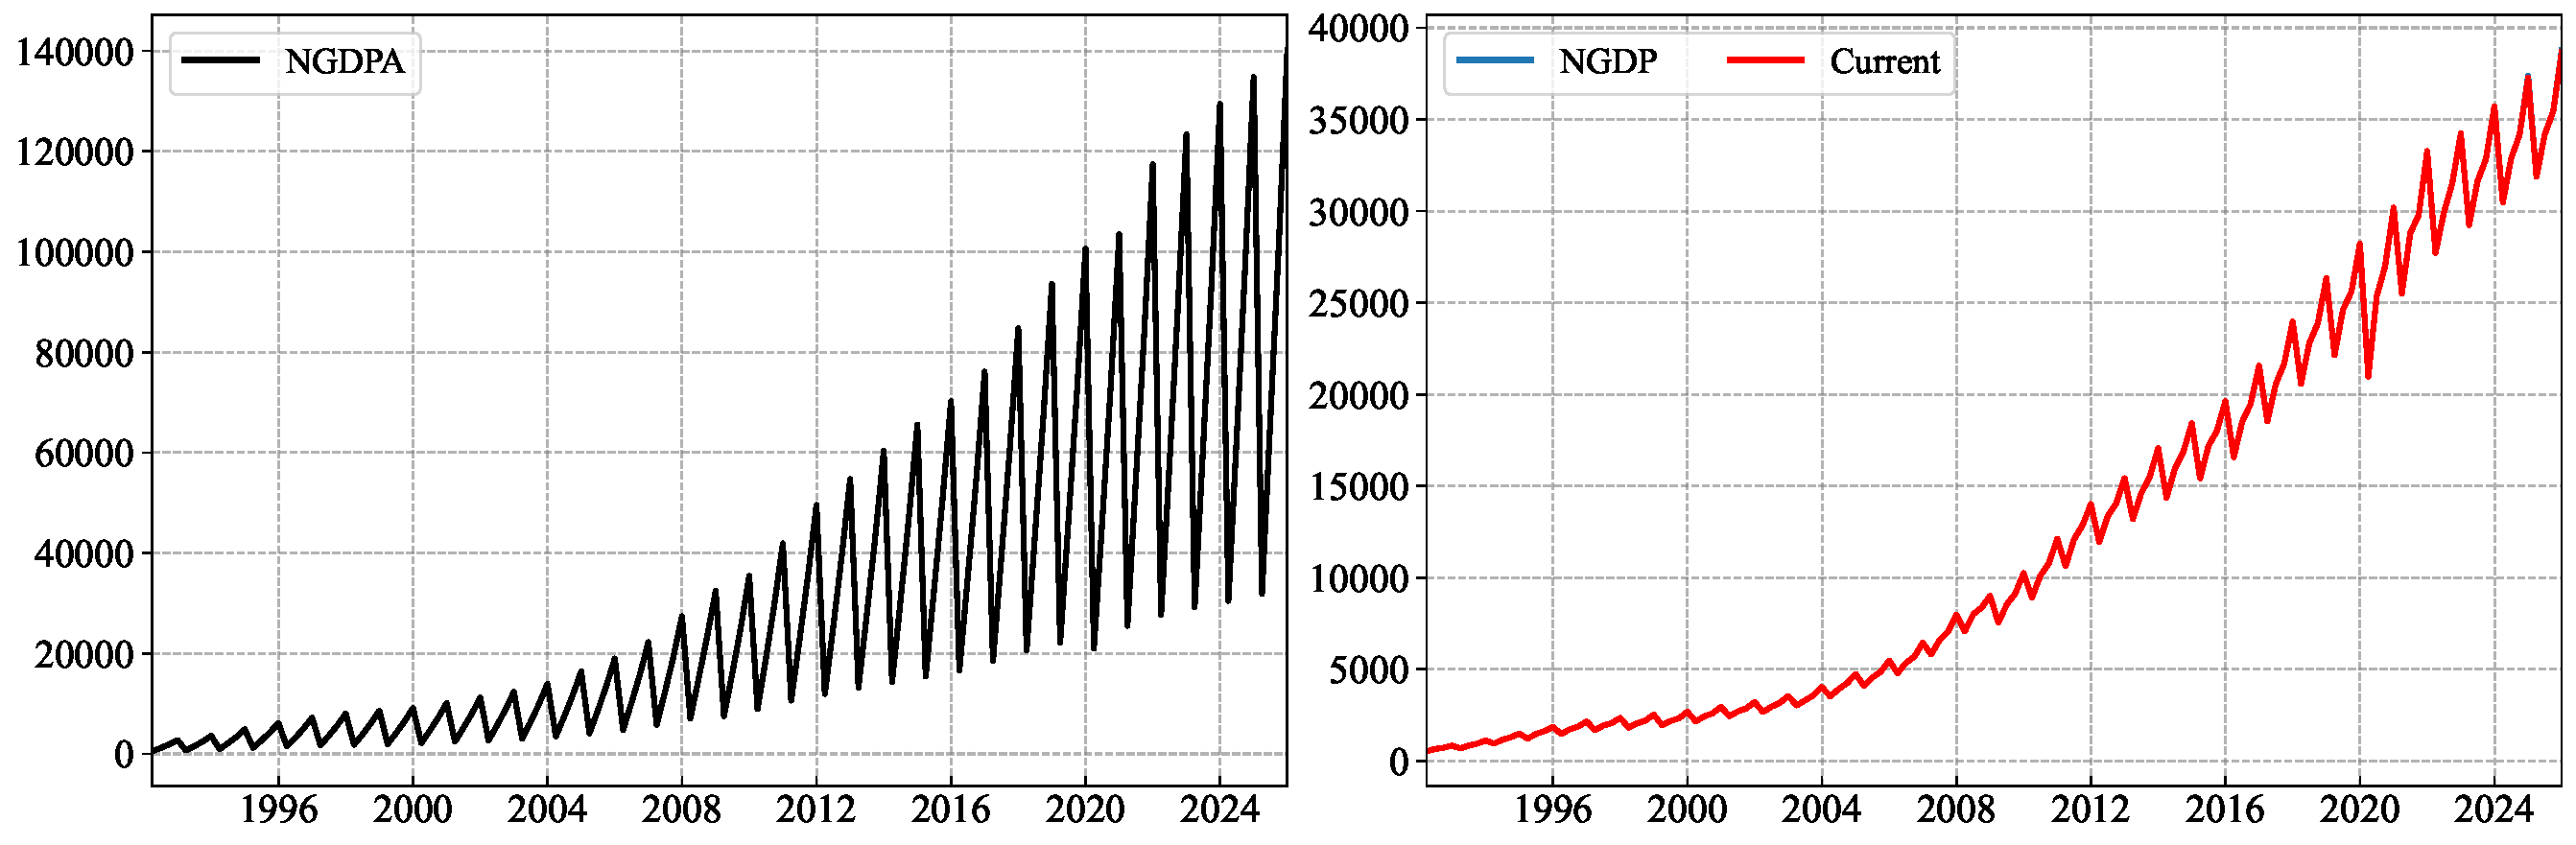
\includegraphics[width=1\linewidth]{figure/Accumulated2Current.pdf}
			\label{fig:Accumulated2Current}
			\vspace{-10pt}
			\caption*{\footnotesize \textit{Notes}: Conversion from cumulative to flow values: the left panel shows China’s year-to-date cumulative nominal GDP, while the right panel reports the corresponding quarterly nominal GDP flow series constructed from successive within-year differences of the cumulative series.}
		\end{figure}
		
		\begin{figure}[htbp]
			\centering
			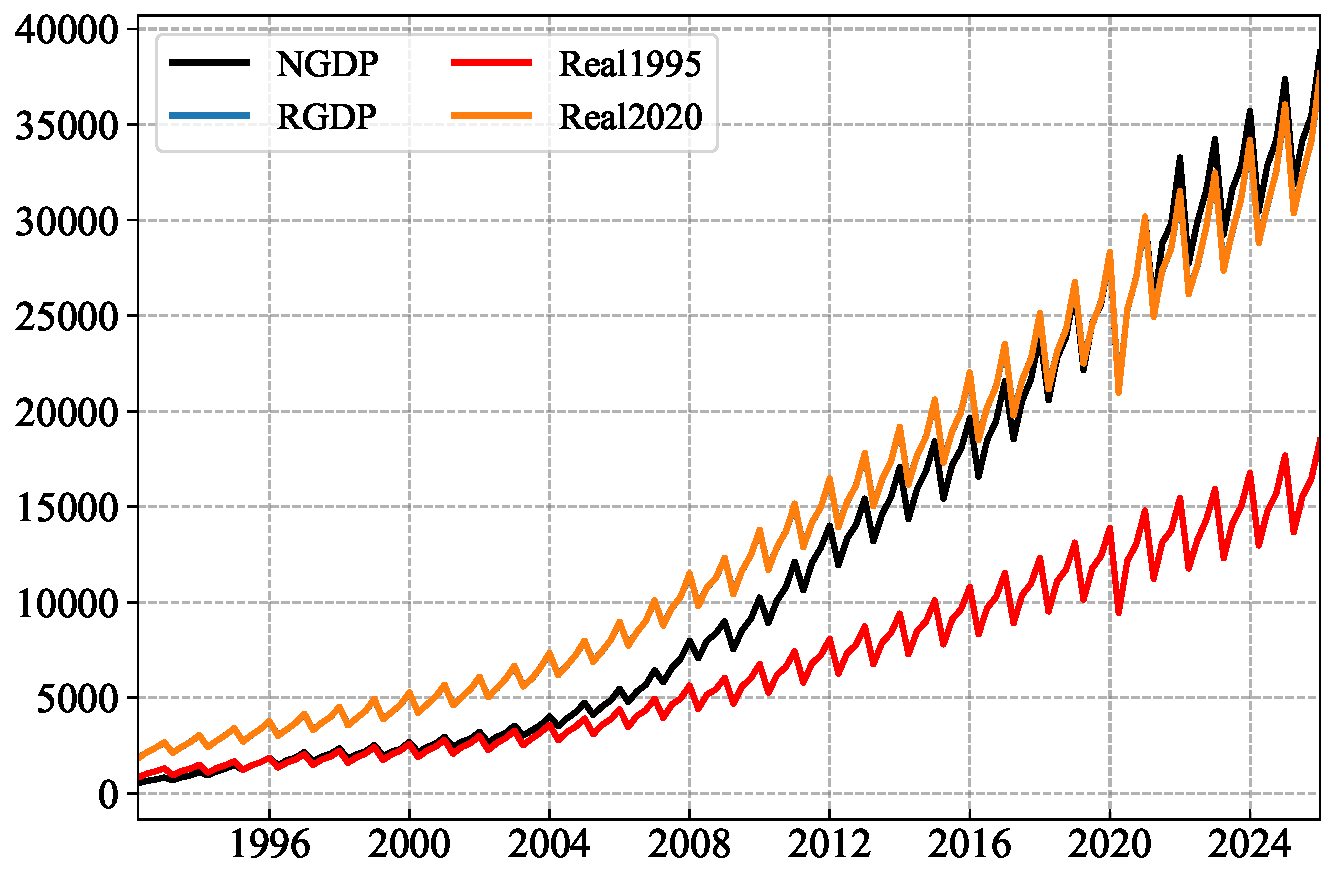
\includegraphics[width=0.55\linewidth]{figure/Norminal2Real.pdf}
			\label{fig:Norminal2Real}		
			\caption*{\footnotesize \textit{Notes}: Conversion from nominal to real values: the black solid line shows nominal GDP, whereas the red and orange solid lines report real GDP series constructed under different base years while preserving the same year-on-year growth profile.}
		\end{figure}
		
		\begin{figure}[htbp]
			\centering
			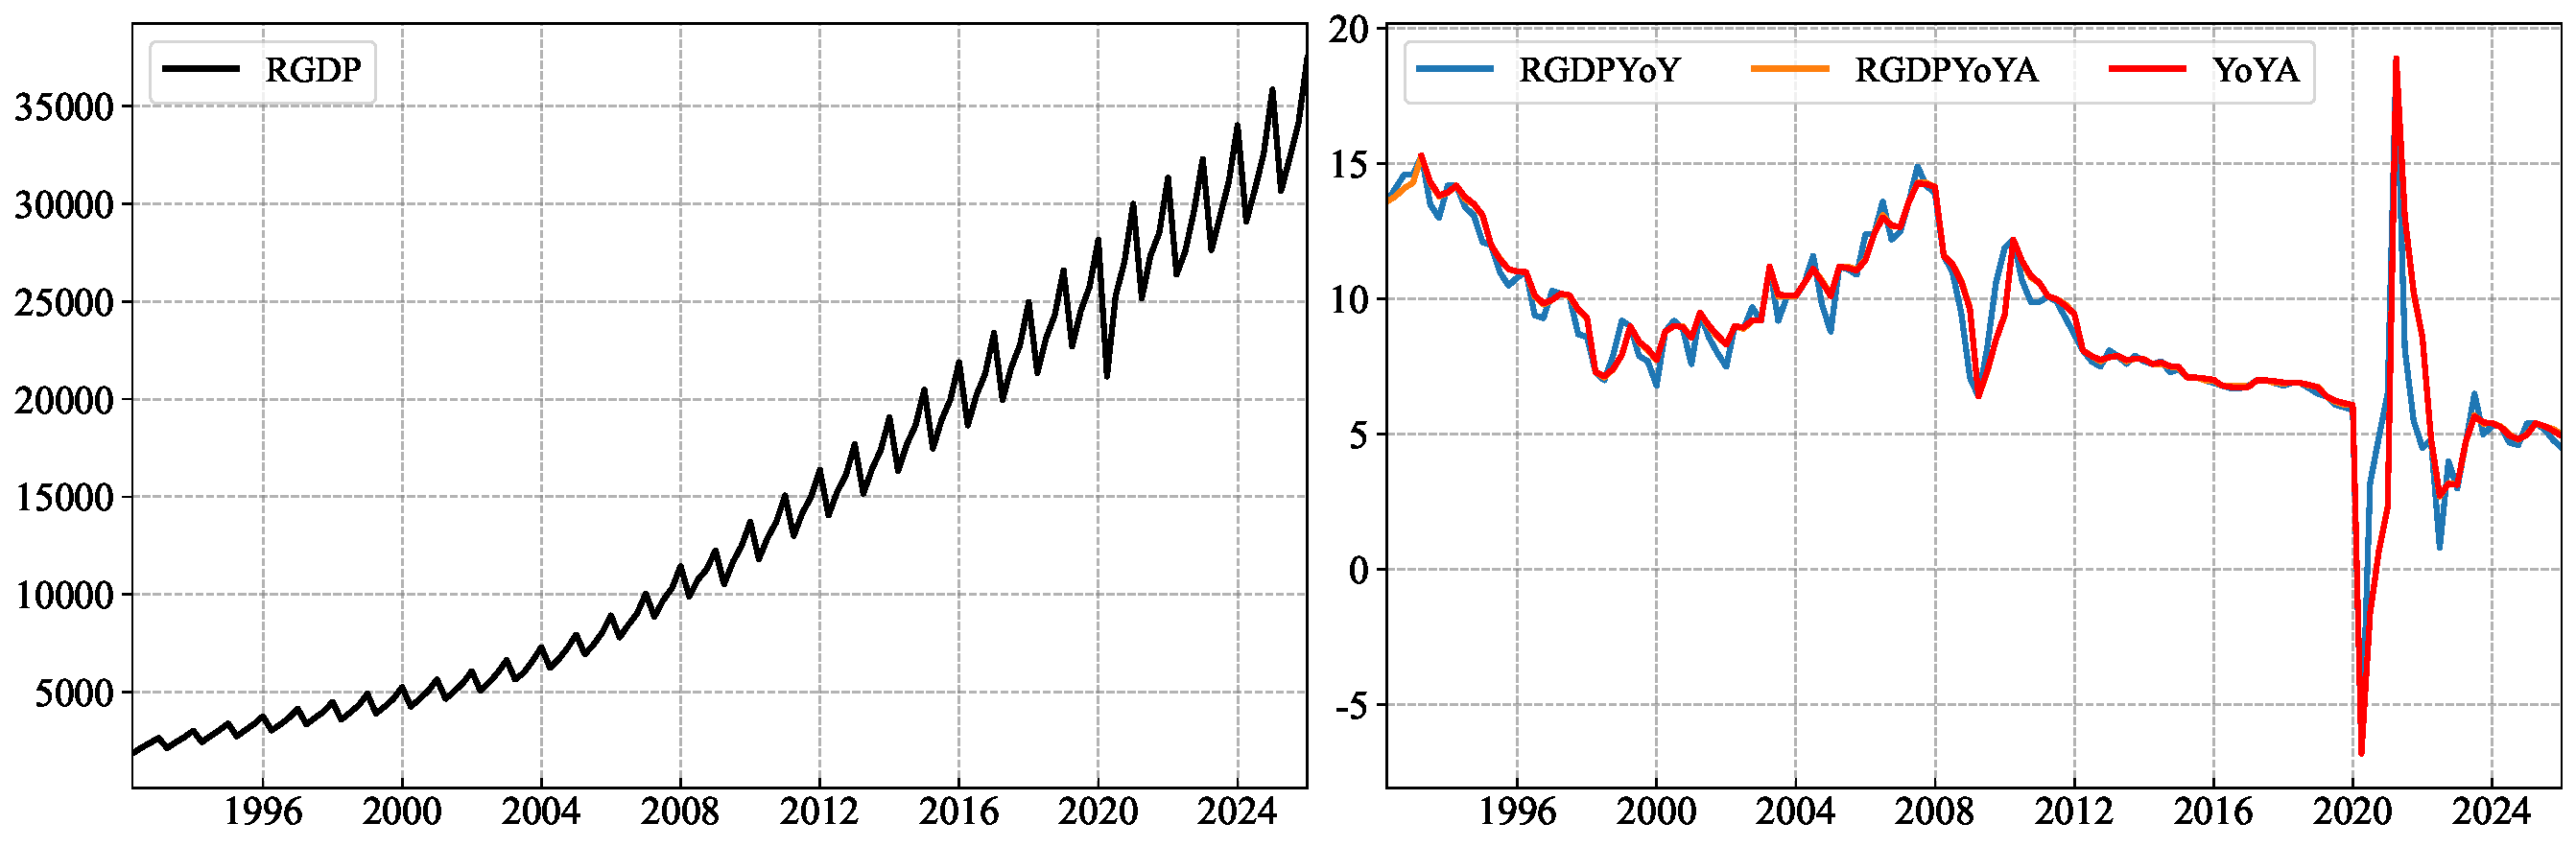
\includegraphics[width=1\linewidth]{figure/Current2AccumulatedYoY.pdf}
			\label{fig:Current2AccumulatedYoY}
			\vspace{-10pt}
			\caption*{\footnotesize \textit{Notes}: Year-on-year growth versus cumulative year-on-year growth: the left panel plots real GDP at 2020 constant prices, while in the right panel the red solid line denotes the cumulative year-on-year growth rate and the blue solid line denotes the year-on-year growth rate. The figure shows clearly that the cumulative year-on-year growth rate is comparatively smoother.}
		\end{figure}
		
		\begin{figure}[htbp]
			\centering
			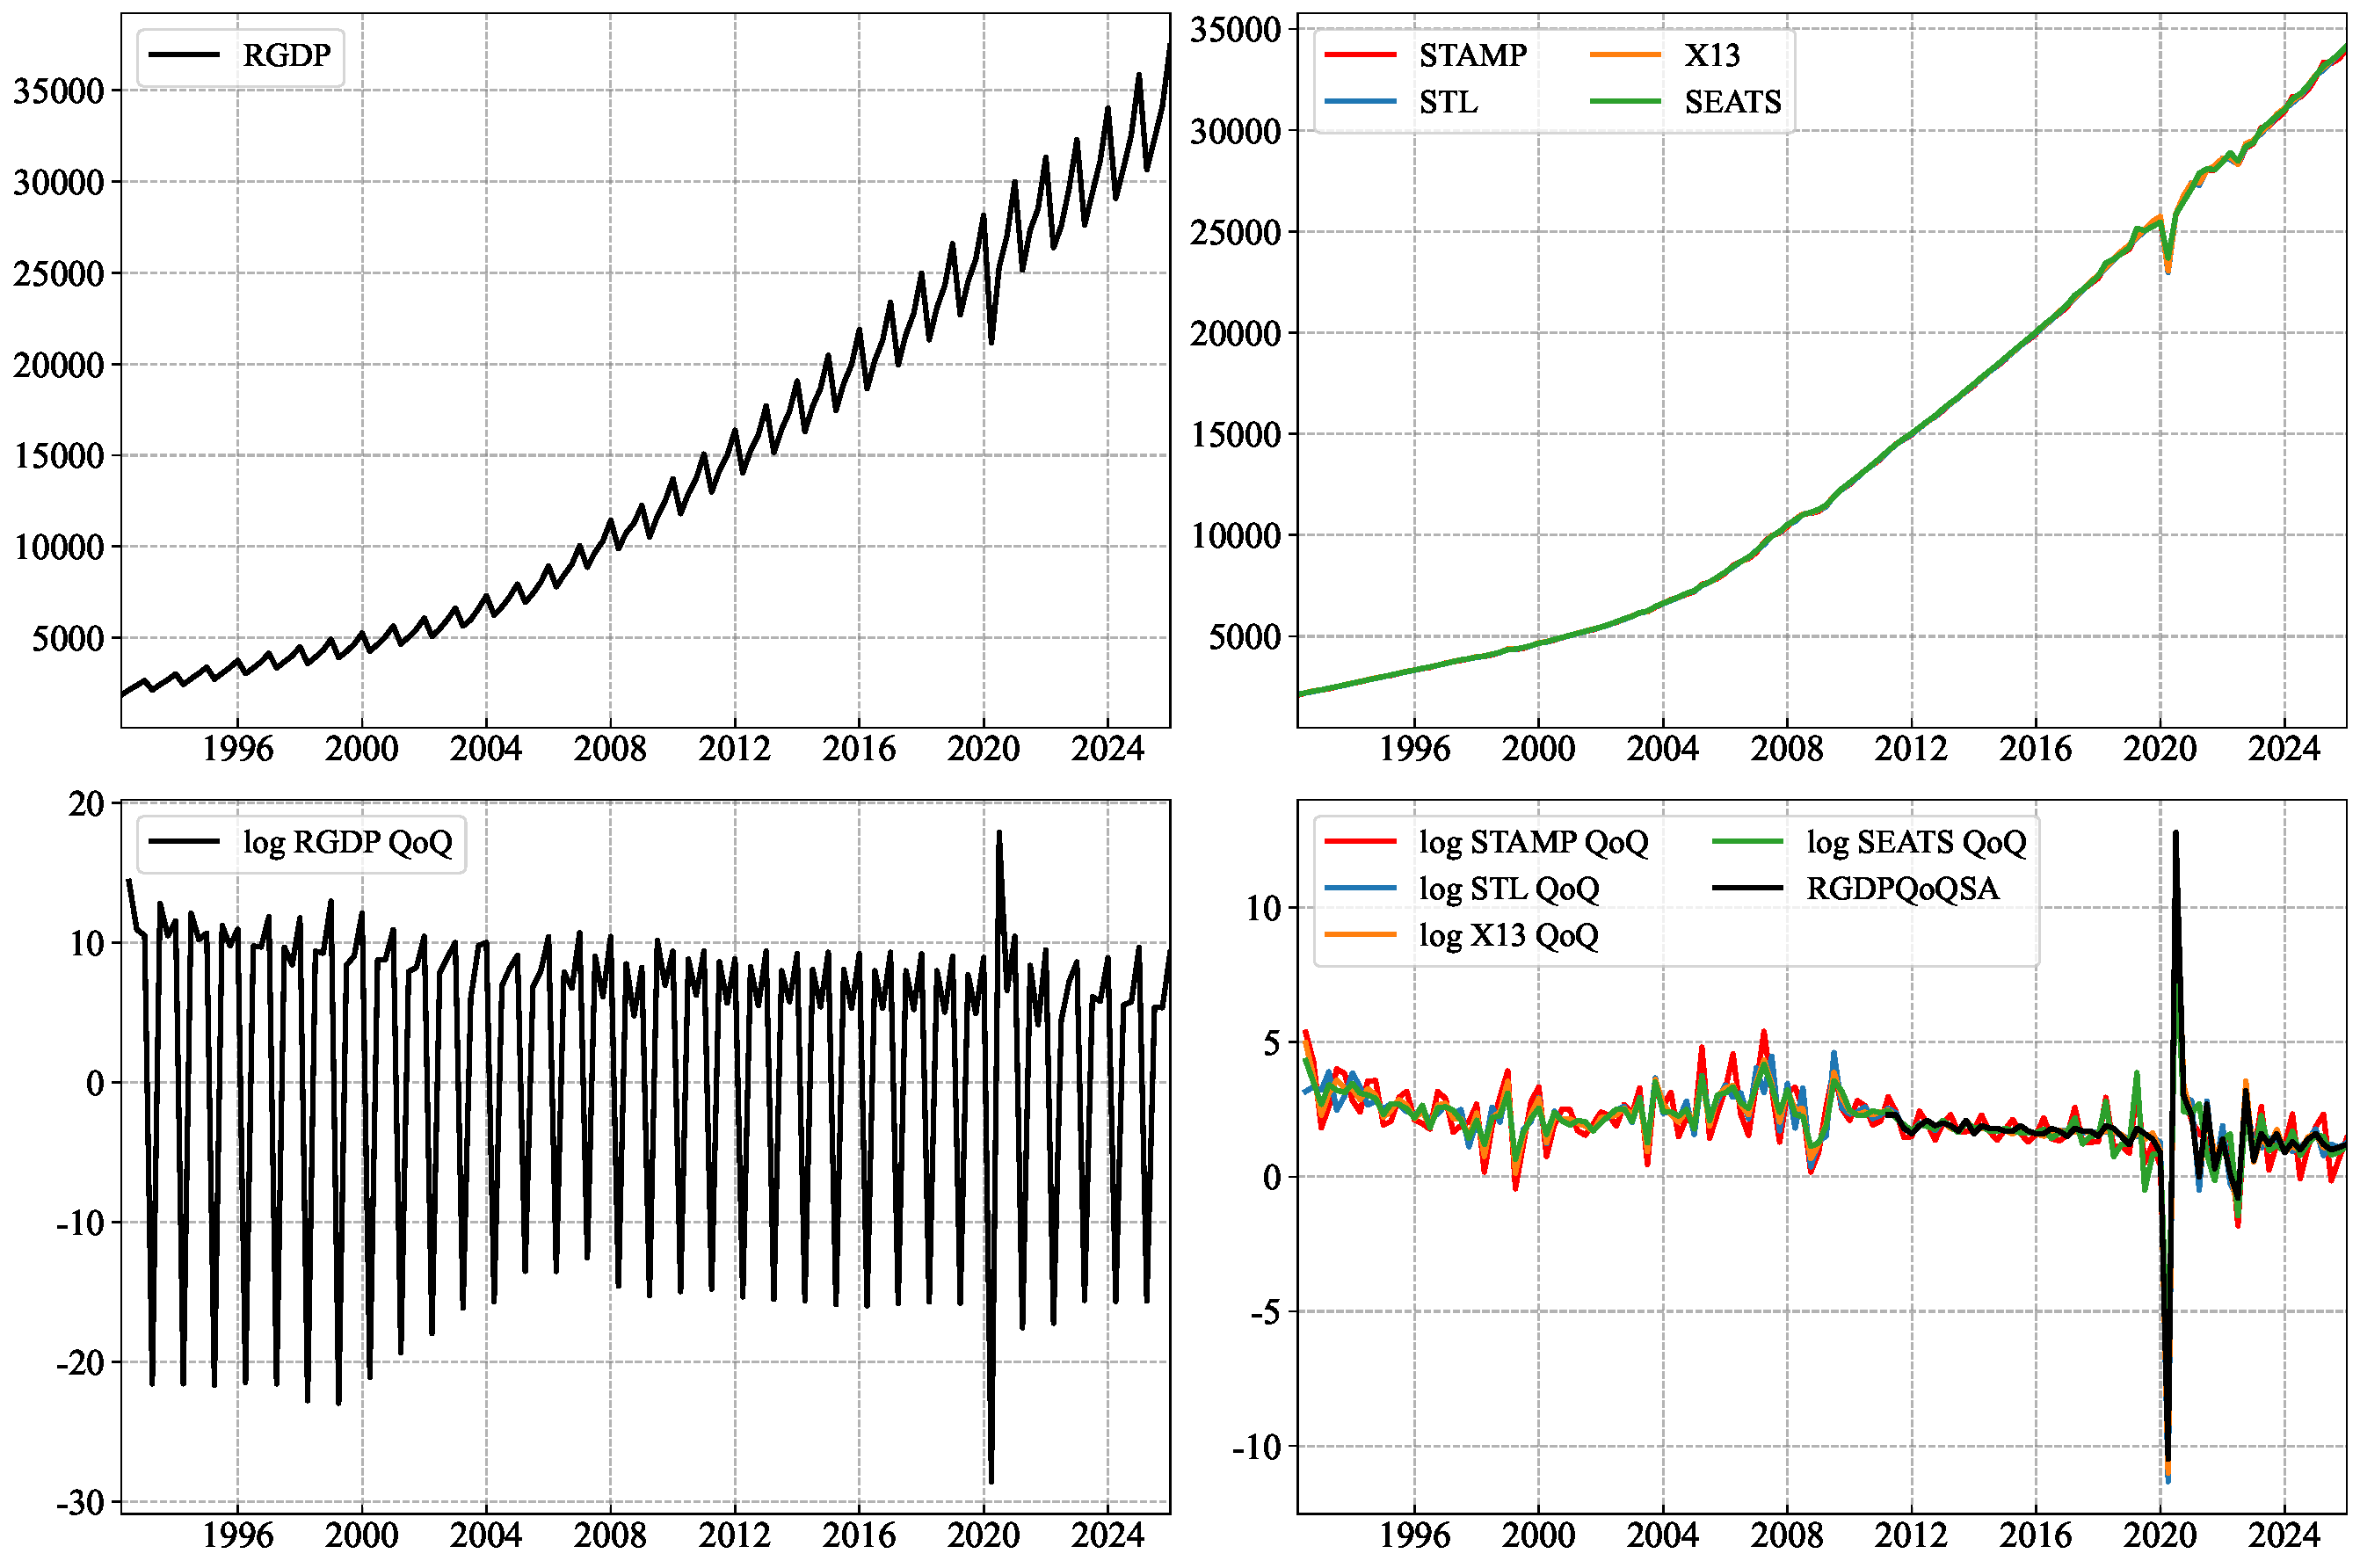
\includegraphics[width=1\linewidth]{figure/SeasonalAdjustment.pdf}
			\label{fig:SeasonalAdjustment}
			\vspace{-10pt}
			\caption*{\footnotesize \textit{Notes}: Seasonal adjustment: the upper-left panel shows quarterly GDP at 2020 constant prices. Directly computed log quarter-on-quarter growth rates, reported in the lower-left panel, display strong seasonal variation and therefore require seasonal adjustment. The upper-right panel presents the seasonally adjusted series obtained from X-13-ARIMA, STL, SEATS and STAMP, while the lower-right panel reports the corresponding log quarter-on-quarter growth rates. The resulting estimates are broadly in line with the official series released by the National Bureau of Statistics after 2012. A particularly striking feature is the exceptionally large fluctuation in China’s growth during the COVID-19 episode in 2020.}
		\end{figure}
		
		\begin{figure}[htbp]
			\centering
			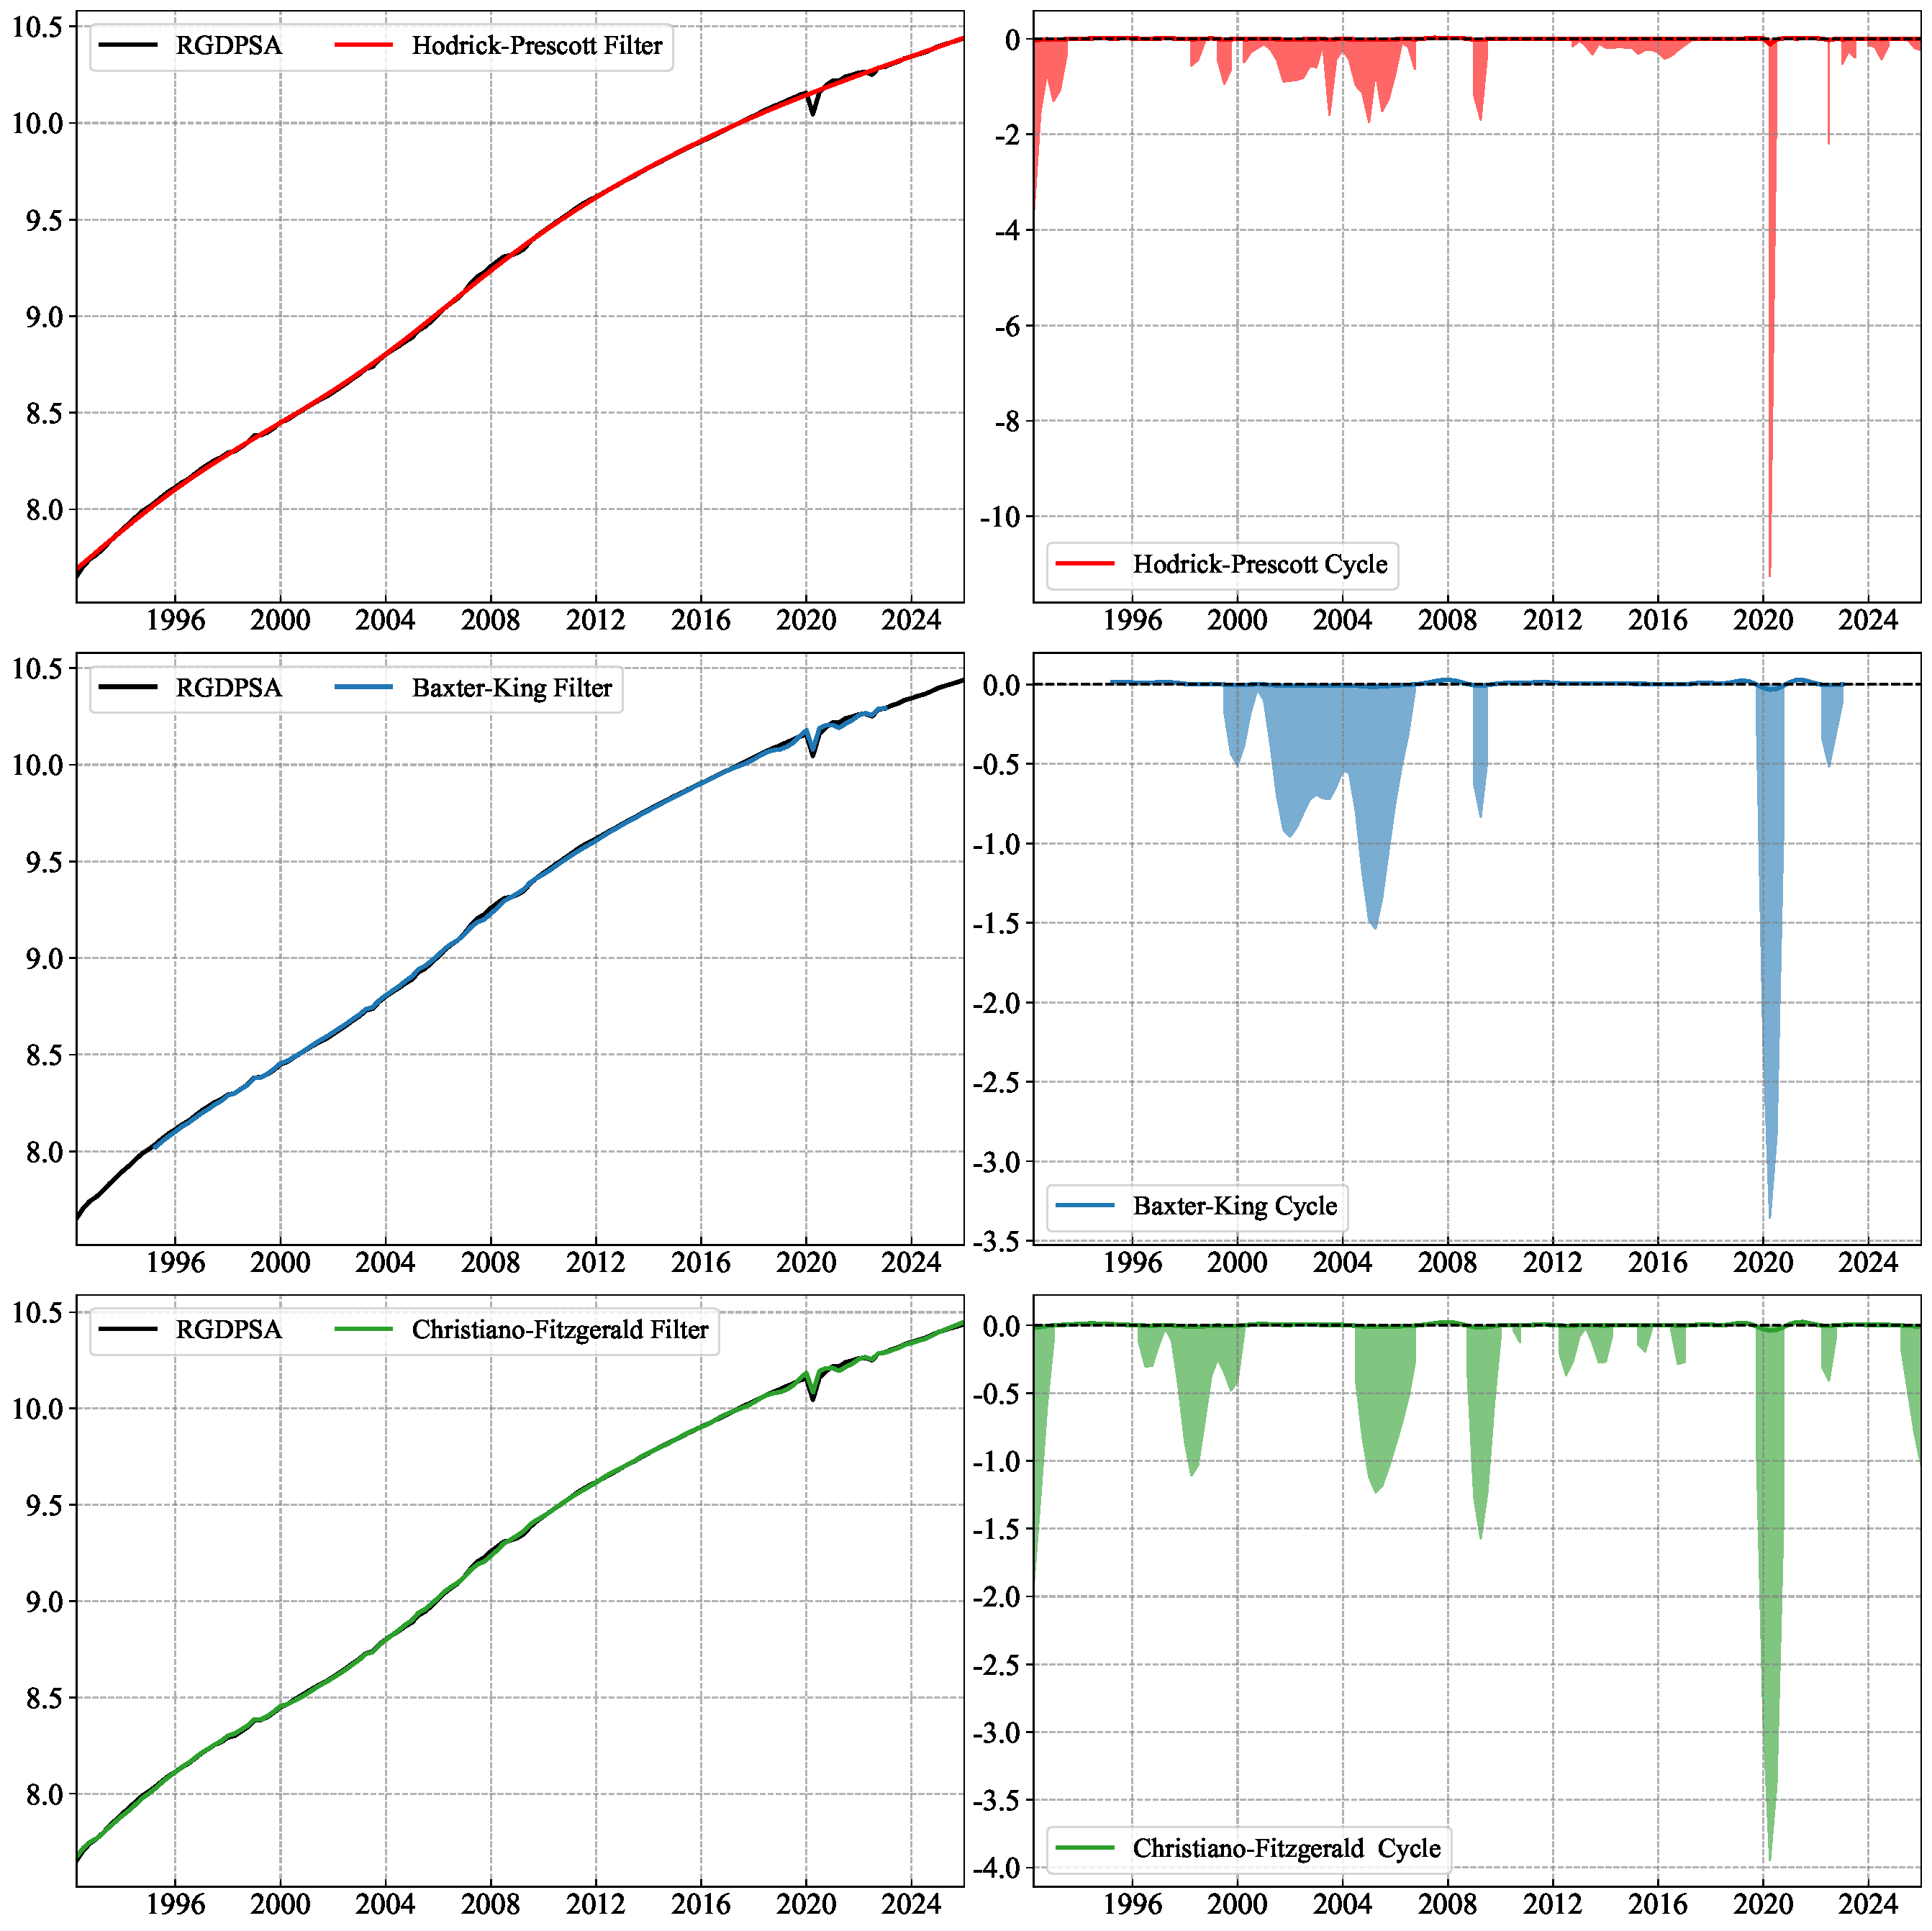
\includegraphics[width=1\linewidth]{figure/TrendCycleDecomposition.pdf}
			\label{fig:TrendCycleDecomposition}
			\vspace{-10pt}
			\caption*{\footnotesize \textit{Notes}: Trend-cycle decomposition: the left panel shows the X-13-ARIMA-adjusted real GDP series together with the trend components extracted by the HP, BK and CF filters, while the right panel reports the corresponding cyclical components. Interpreting the trend as potential output, the cycle provides an approximate measure of the output gap, namely the deviation of actual output from potential output. Positive values indicate a positive output gap, whereas negative values indicate a negative output gap.}
		\end{figure}
		
		\begin{figure}[htbp]
			\centering
			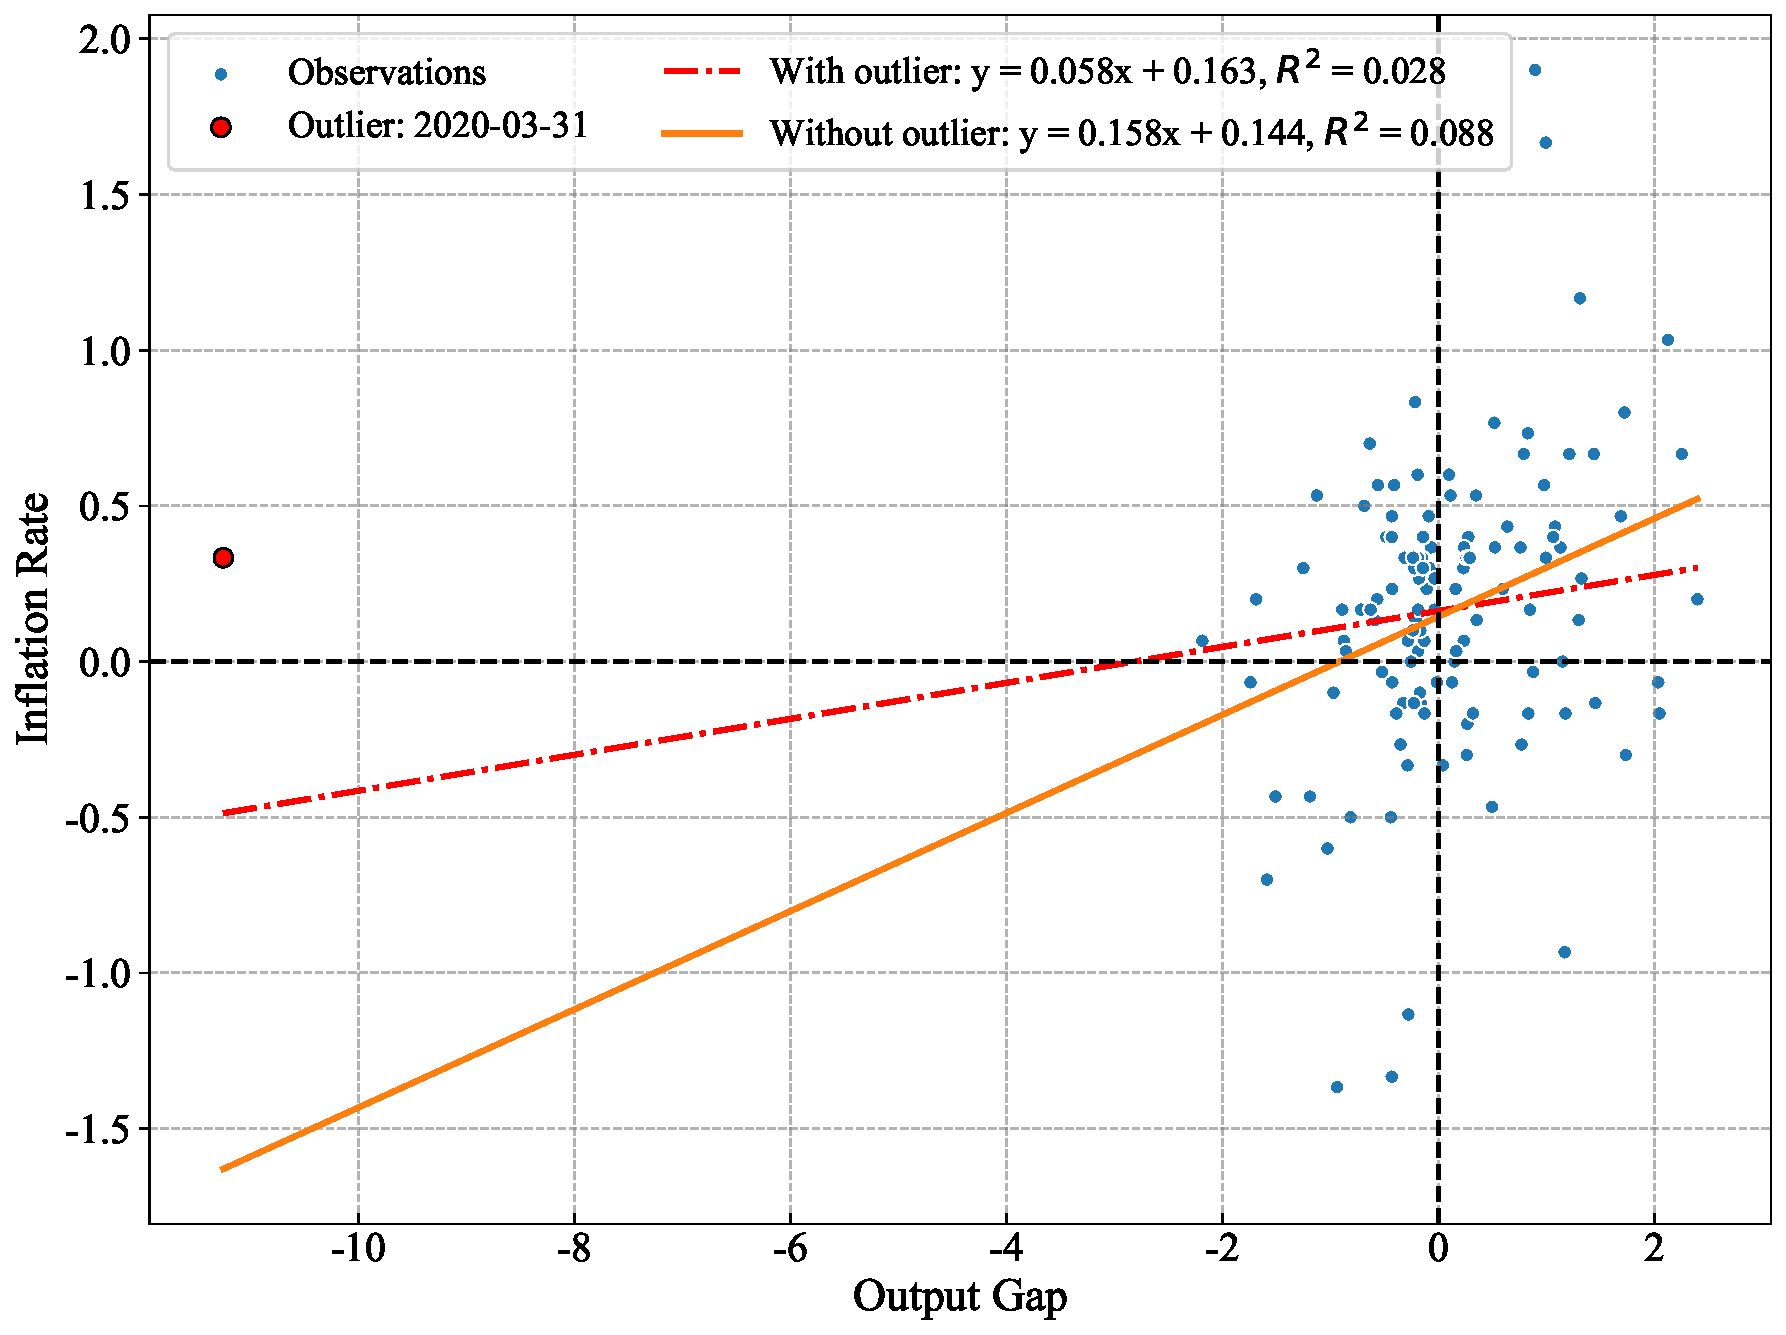
\includegraphics[width=0.85\linewidth]{figure/PhillipsCurve.pdf}
			\label{fig:PhillipsCurve}
			\vspace{-10pt}
			\caption*{\footnotesize \textit{Notes}: Inflation and the output gap: the upper panel plots inflation, measured by CPI month-on-month growth, against the HP-filter-based output gap. The red dash-dotted line denotes the fitted relationship including the extreme observation from March 2020, while the orange solid line excludes that observation. The fitted lines indicate a positive association between the output gap and inflation, suggesting that stronger-than-potential economic activity is accompanied by greater inflationary pressure. This result is broadly consistent with a Phillips-curve-type relationship, although it also highlights the sensitivity of the fit to extreme observations.}
		\end{figure}
		
		\begin{figure}[htbp]
			\centering
			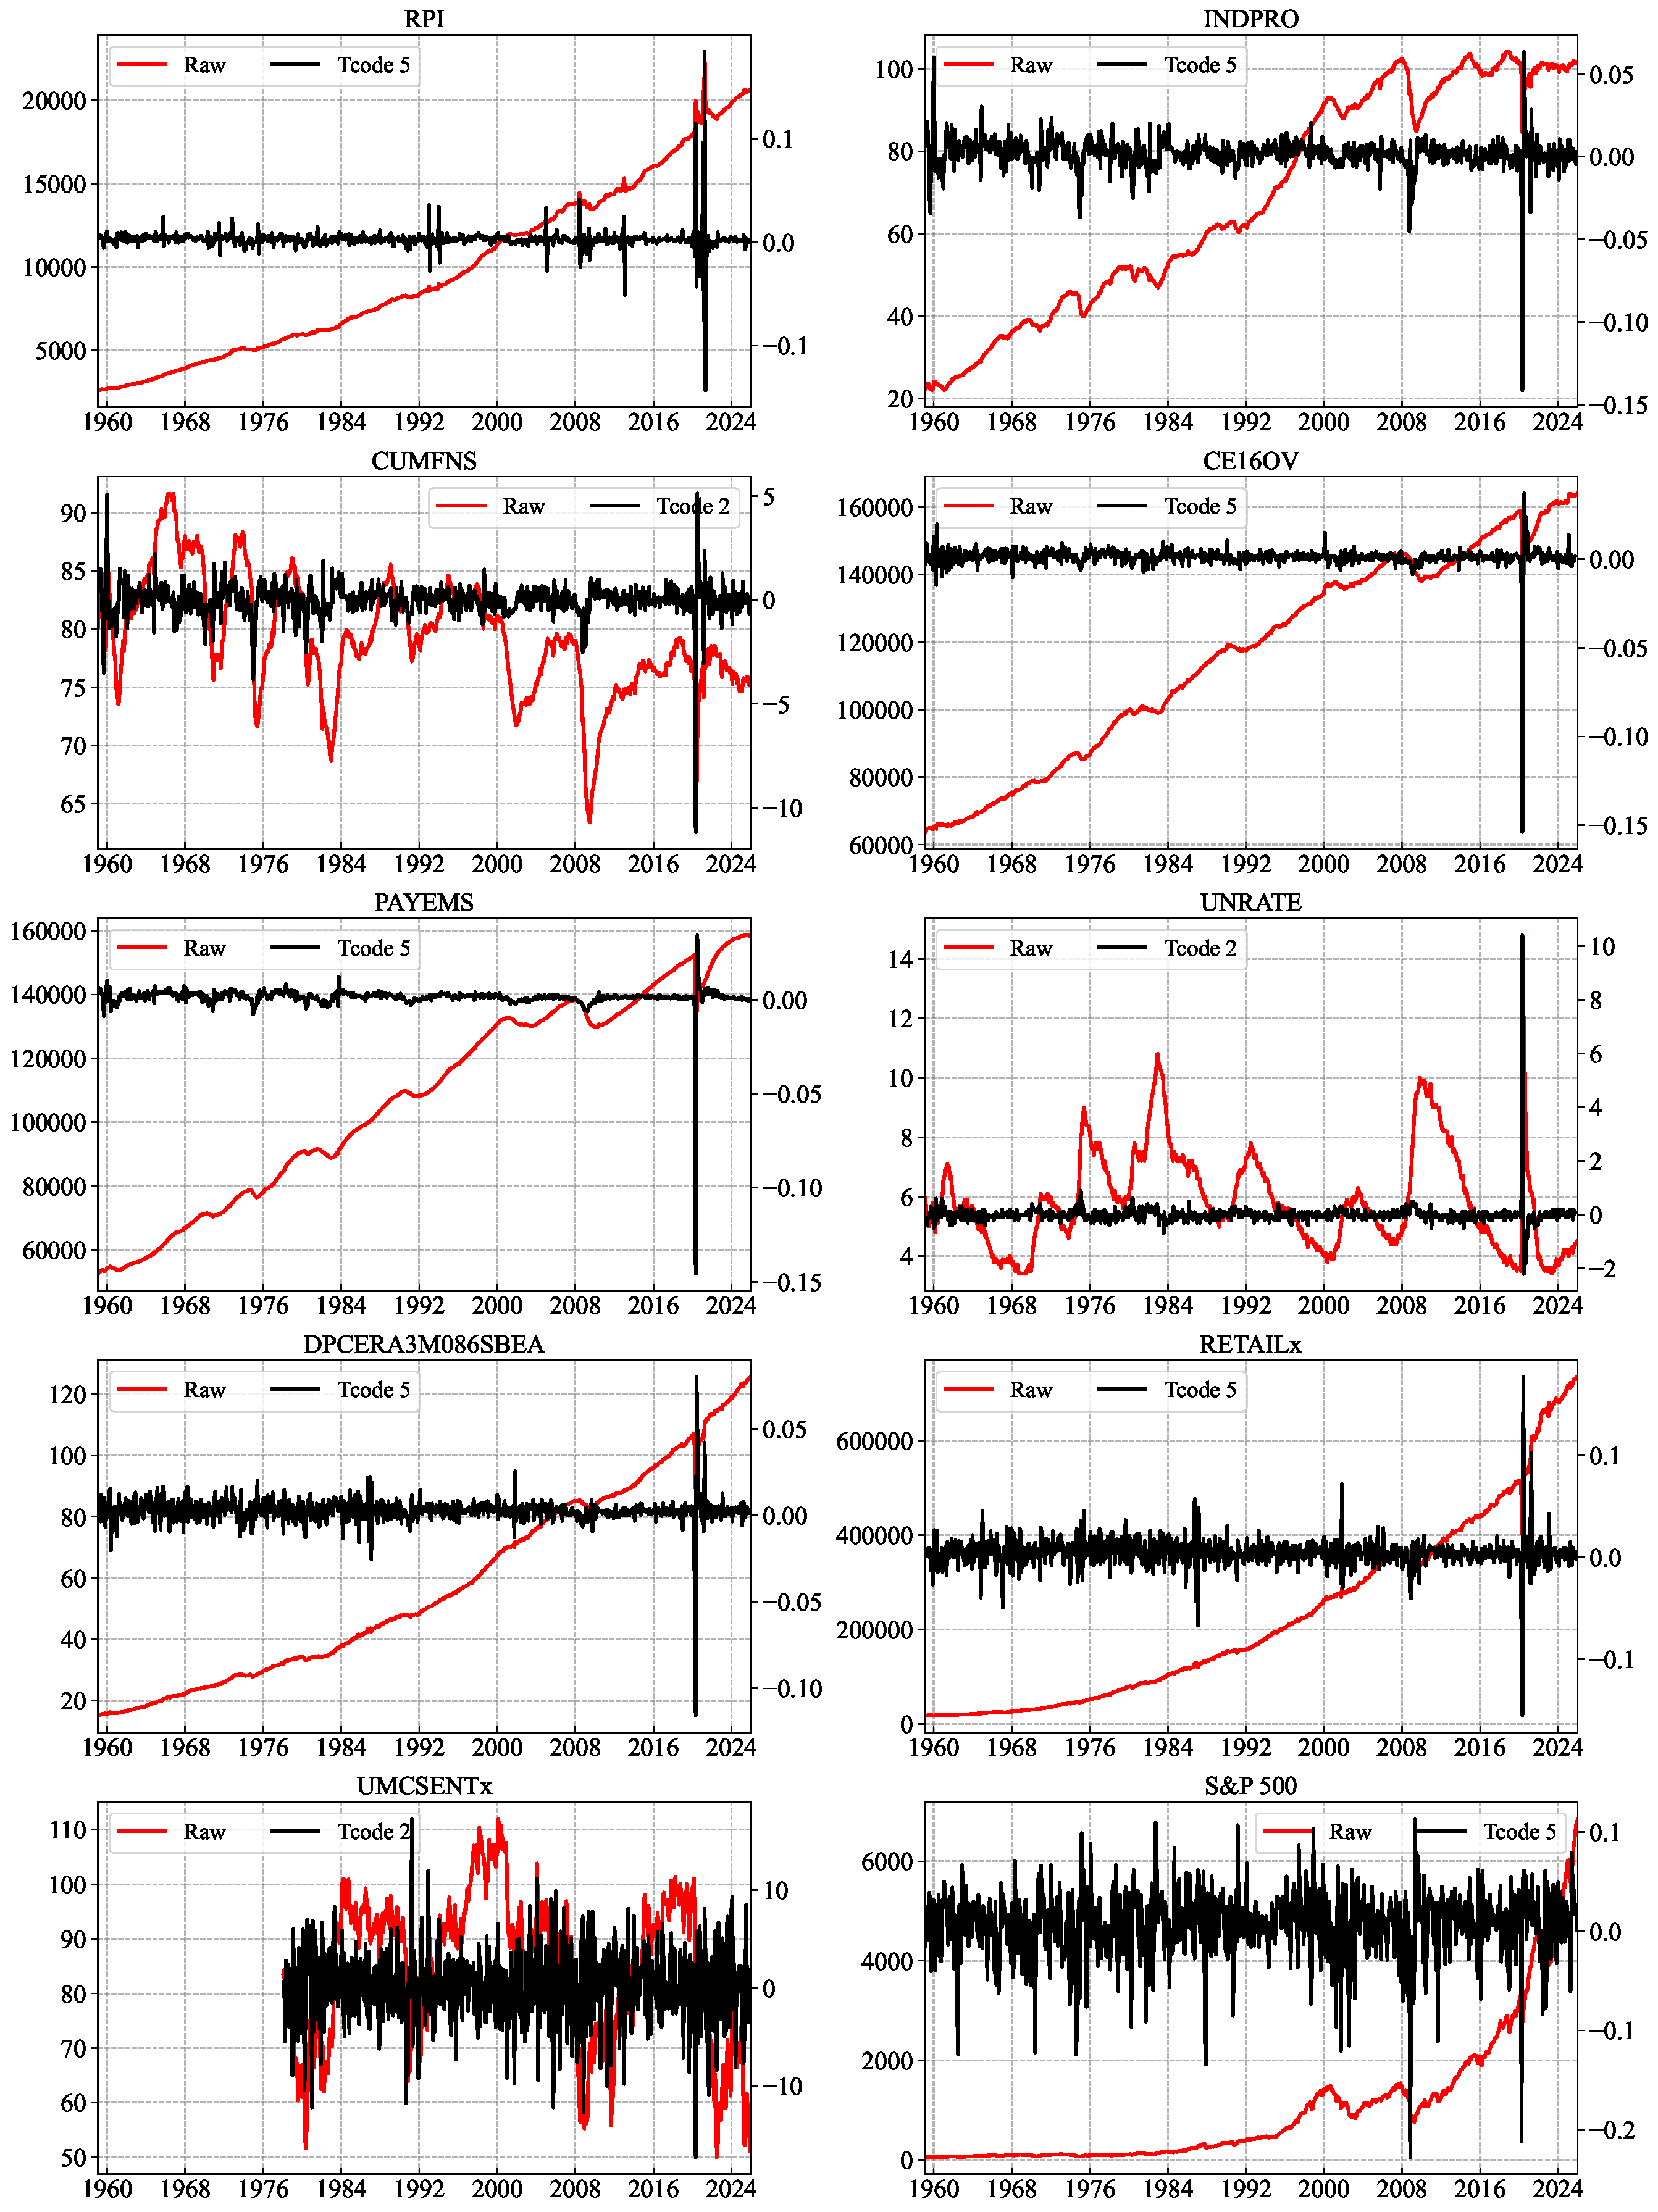
\includegraphics[width=1\linewidth]{figure/FREDTransform.pdf}
			\label{fig:FREDTransform}
			\vspace{-10pt}
			\caption*{\footnotesize \textit{Notes}: FRED-MD is a widely used monthly database for empirical macroeconomic research in the United States. Introduced by McCracken and Ng (2016) in the Journal of Business and Economic Statistics, it groups roughly 120 monthly macroeconomic indicators into eight broad categories, such as output and income, labor market conditions, and the housing sector. The ten-variable subset considered in this assignment is more closely aligned with macroeconomic forecasting applications, and the associated transformations are primarily based on log month-on-month growth rates.}
		\end{figure}

		\begin{figure}[htbp]
			\centering
			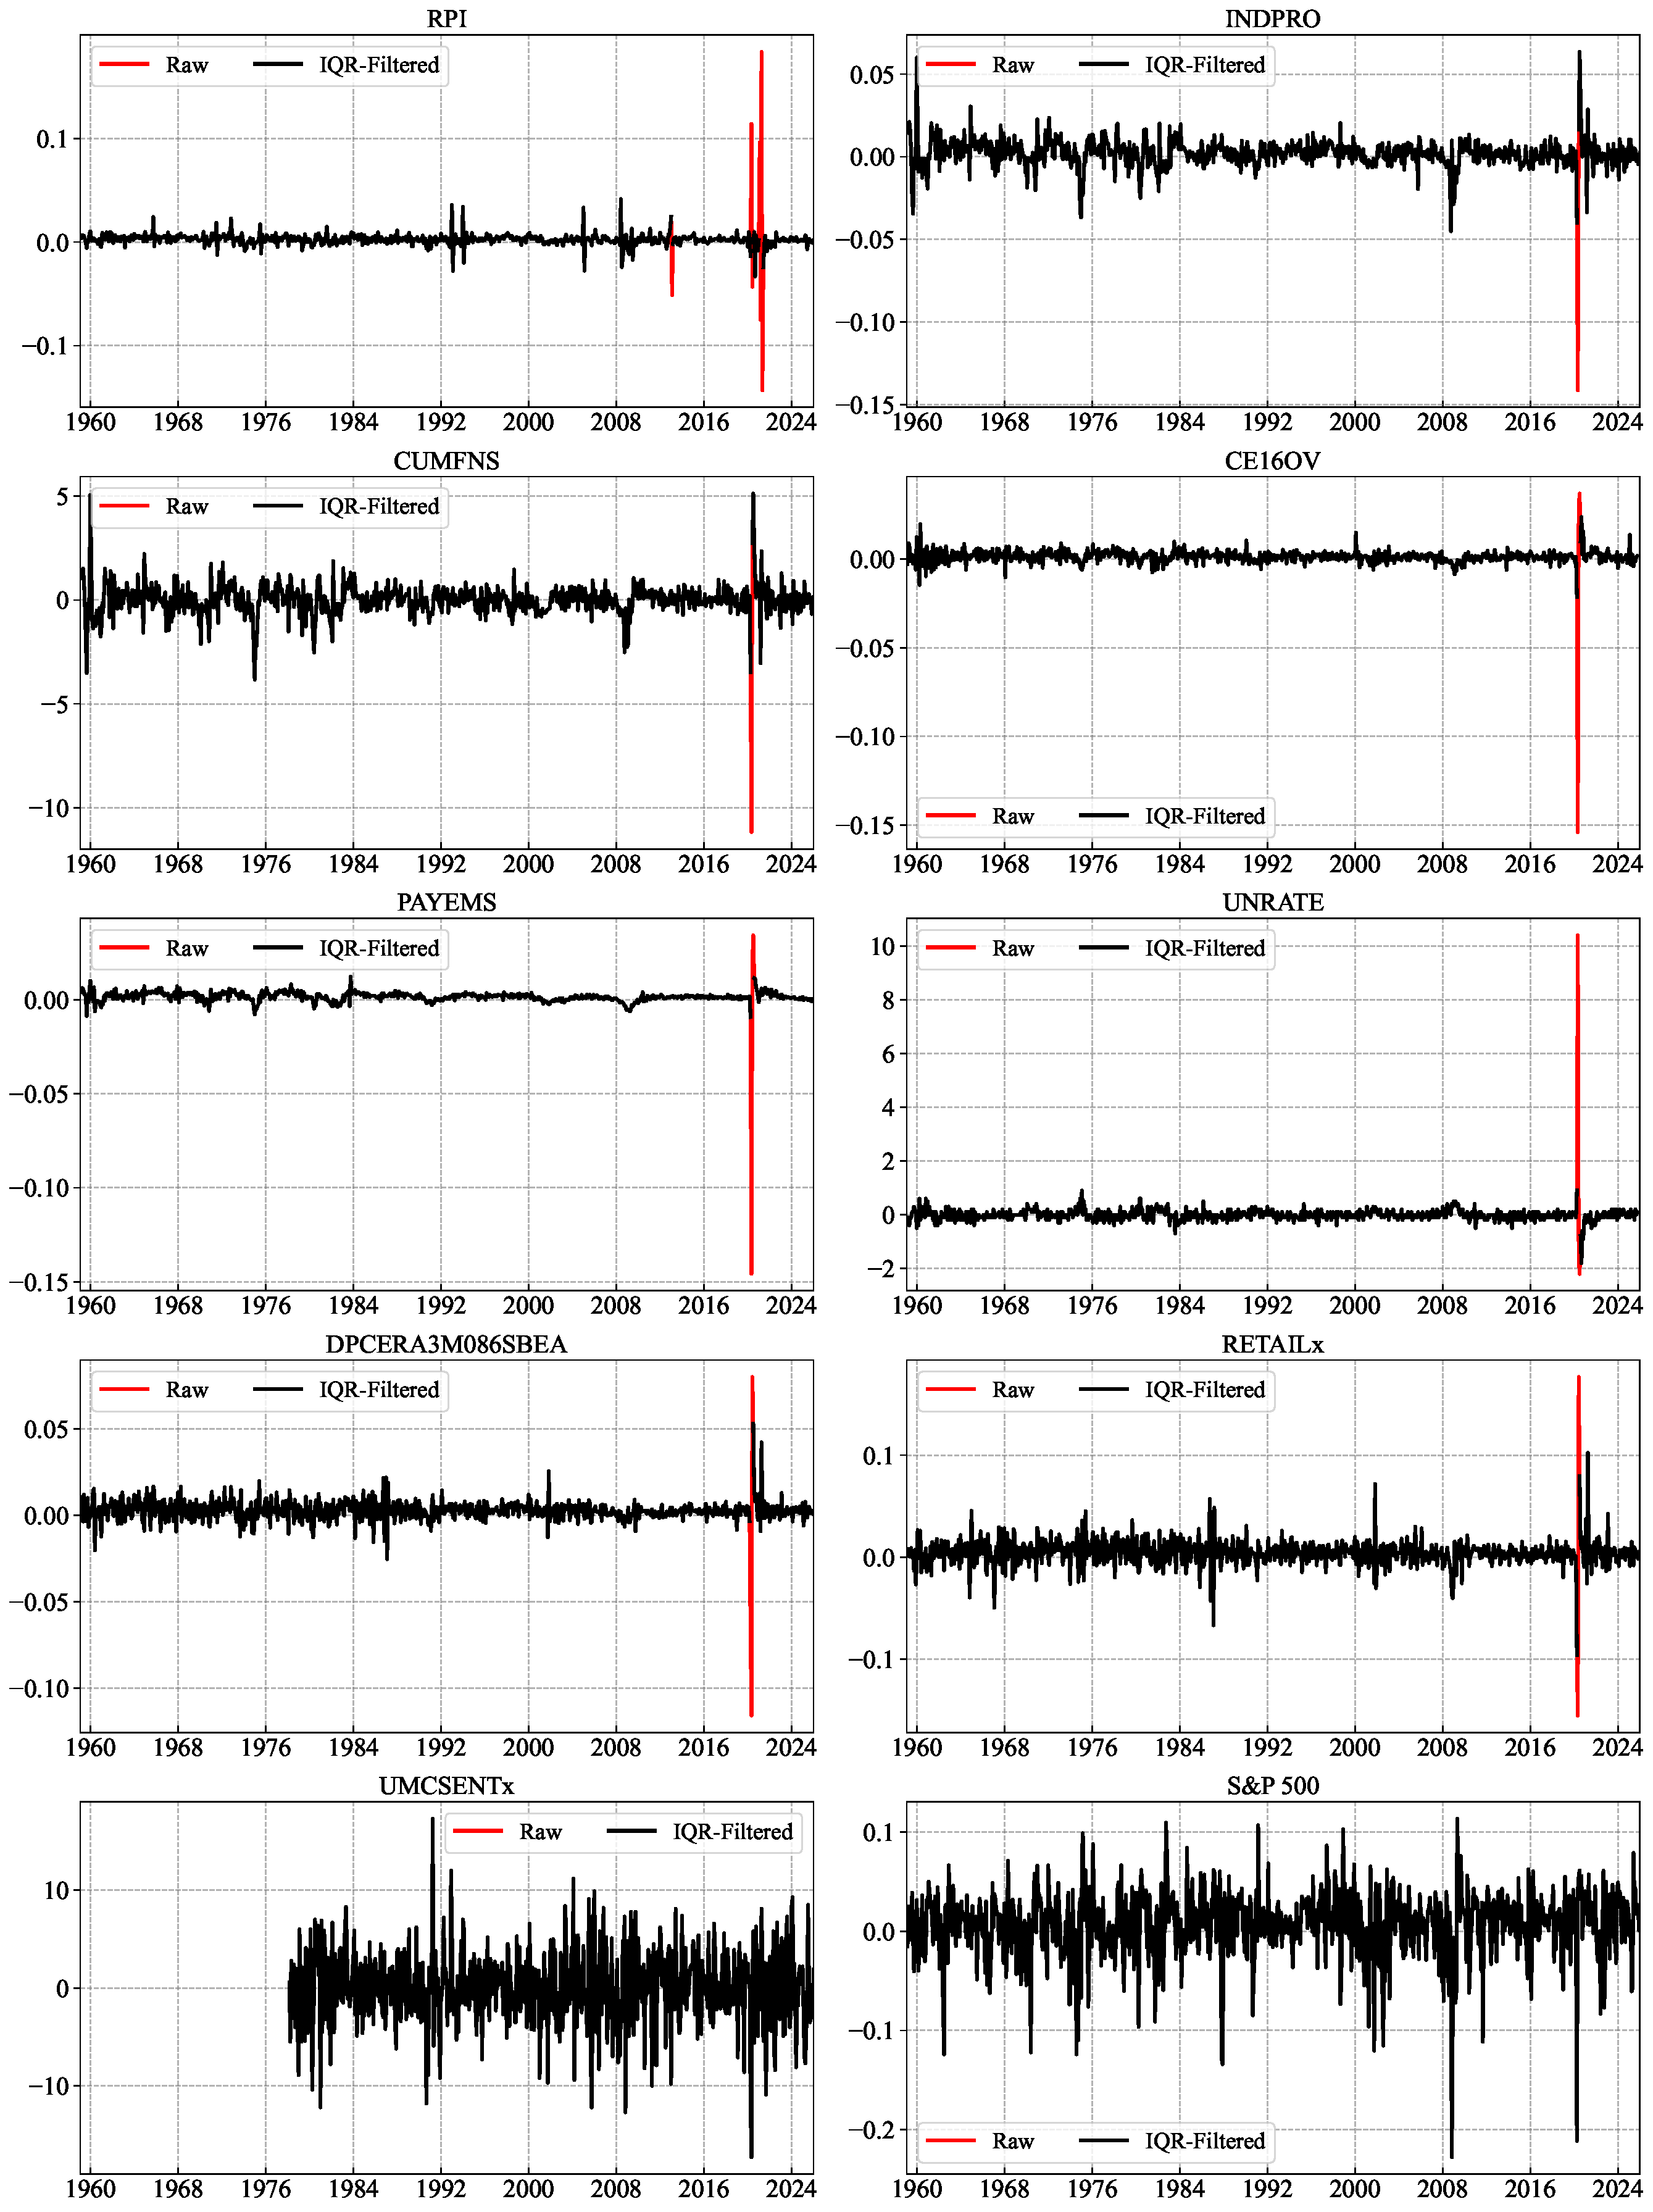
\includegraphics[width=1\linewidth]{figure/OutliersRemoved.pdf}
			\label{OutliersRemoved}
			\vspace{-10pt}
			\caption*{\footnotesize \textit{Notes}: Outlier adjustment: following McCracken and Ng (2016), extreme observations in the stationarized series are identified using the IQR rule. The red solid line plots the original stationary series, whereas the black solid line plots the series after extreme-outlier treatment. The figure shows that the COVID-19 period generated unusually large and historically unprecedented macroeconomic fluctuations in the United States, which helps explain why conventional forecasting models often performed poorly during the pandemic.}
		\end{figure}
		
		\begin{figure}[htbp]
			\centering
			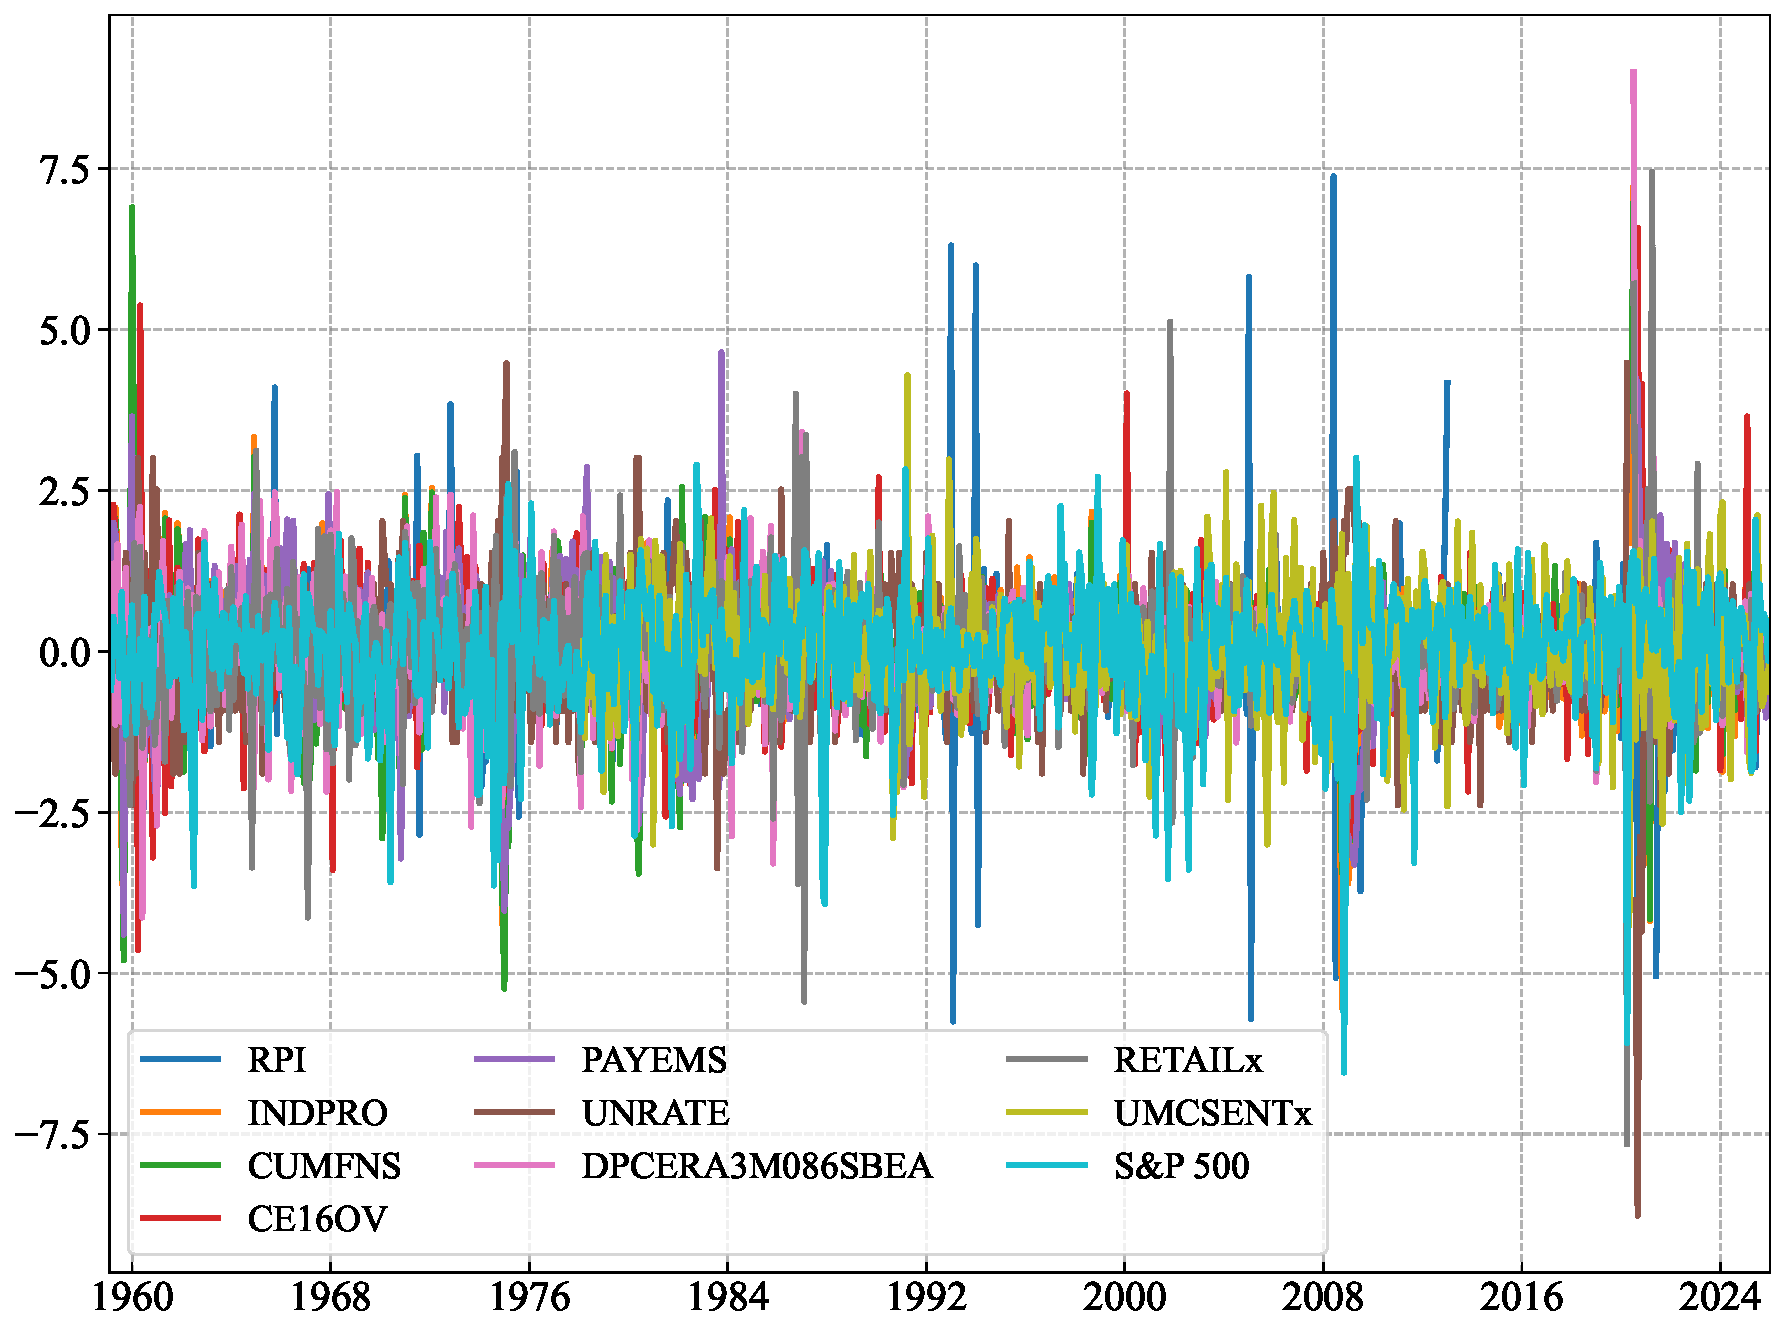
\includegraphics[width=0.85\linewidth]{figure/ZScore.pdf}
			\label{ZScore}
			\vspace{-10pt}
			\caption*{\footnotesize \textit{Notes}: Z-score standardization: because the series differ in units, scale, and volatility, the figure reports the standardized series after extreme outliers have been removed. Standardization facilitates cross-series comparability and subsequent modeling. At the same time, some extreme observations may reflect economically meaningful shocks rather than mere noise, so the treatment of outliers should be guided by the research objective and by the trade-off between statistical robustness and economic interpretation.}
		\end{figure}
		
		\begin{figure}[htbp]
			\centering
			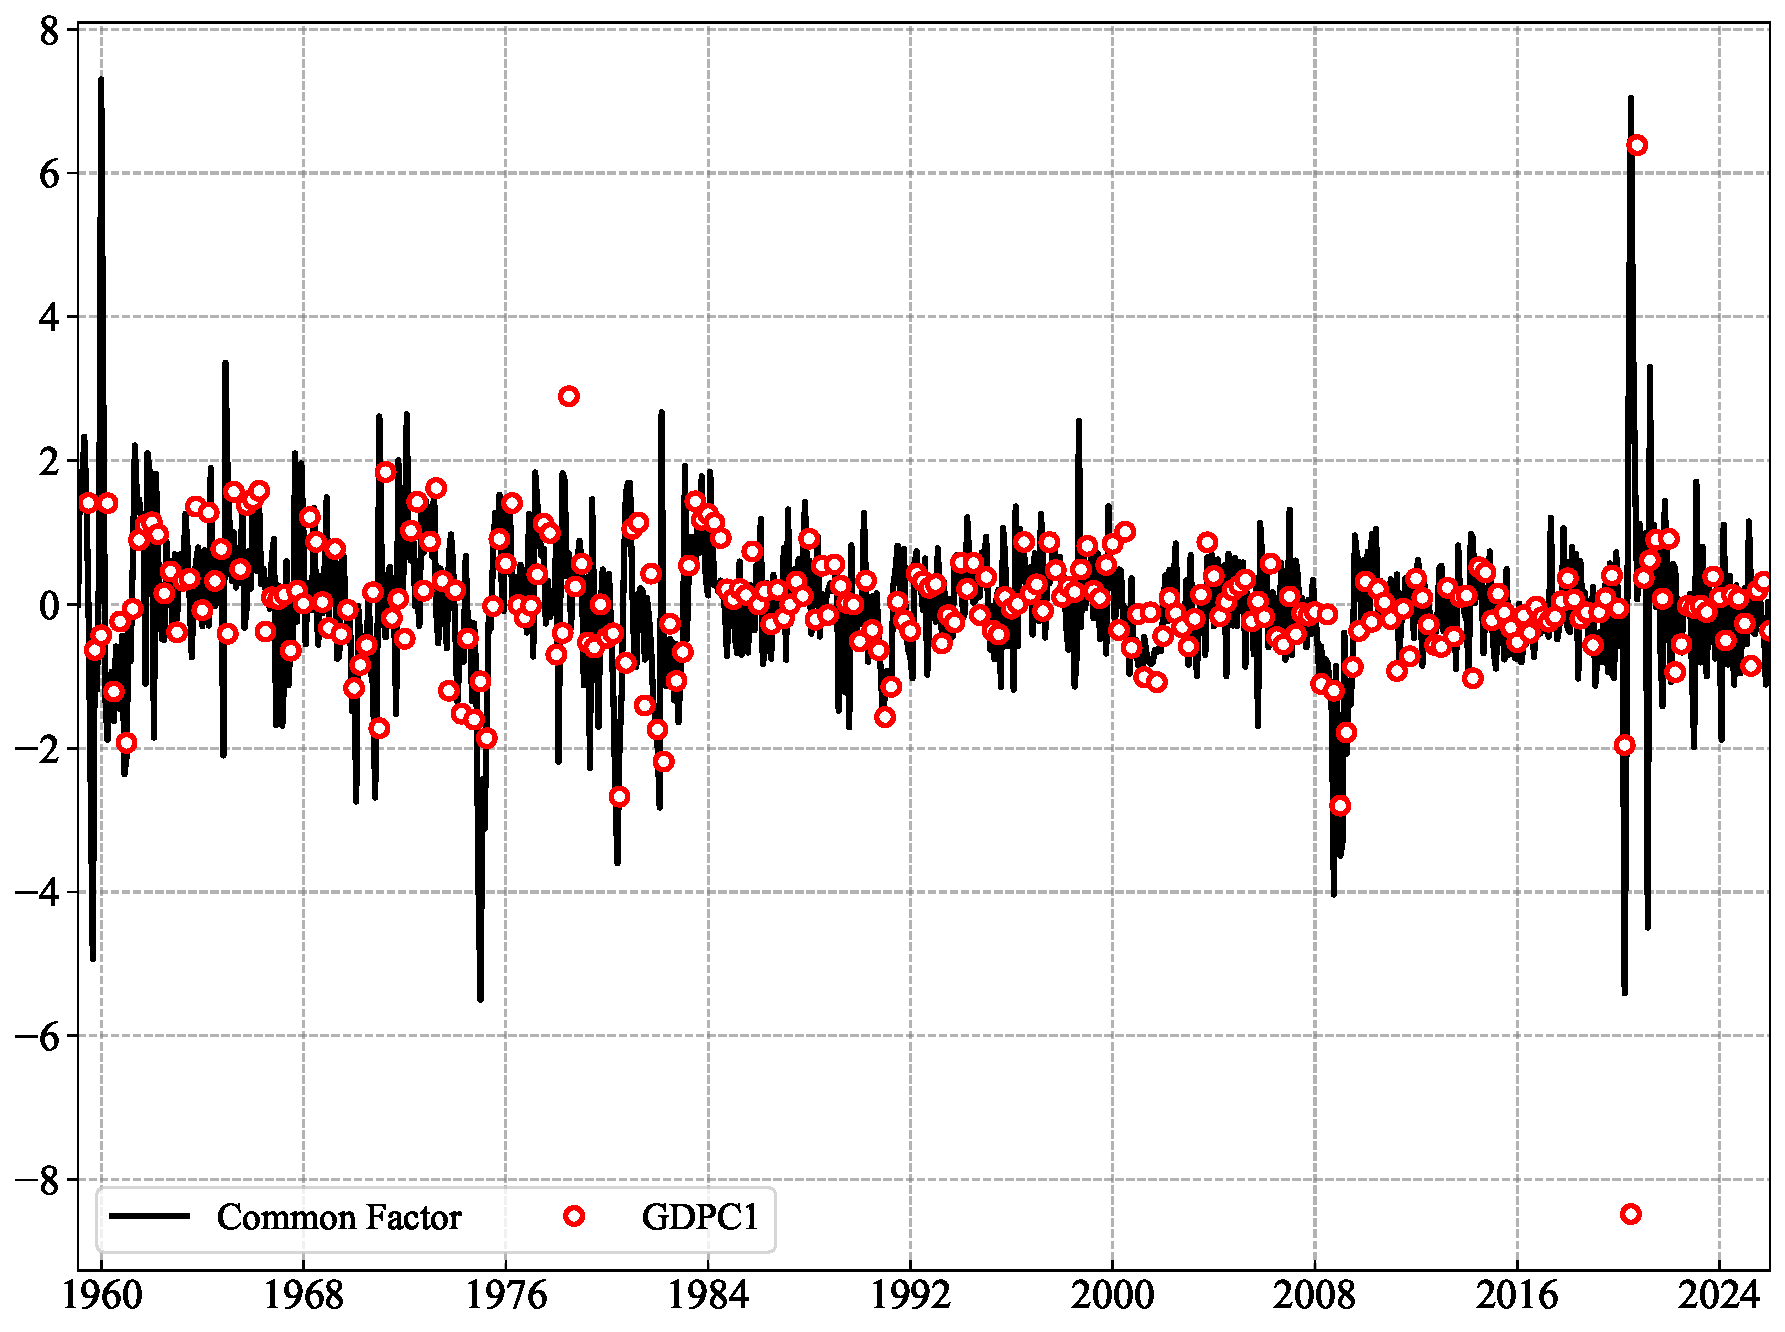
\includegraphics[width=0.85\linewidth]{figure/DynamicFactor.pdf}
			\label{DynamicFactor}
			\vspace{-10pt}
			\caption*{\footnotesize \textit{Notes}: Dynamic factor model: the figure shows the monthly common factor extracted from a dynamic factor model estimated using ten macroeconomic variables, together with quarter-on-quarter GDP growth. The common factor exhibits pronounced comovement with GDP growth, suggesting that higher-frequency monthly information may help track, and potentially nowcast, broader macroeconomic conditions. For the specification and estimation of the dynamic factor model, see the following Statsmodels example: \url{https://www.statsmodels.org/dev/examples/notebooks/generated/statespace_dfm_coincident.html}}
		\end{figure}
	\end{reference}

\end{document}